%%% -*-LaTeX-*-
%\extrafloats{100}

\chapter{Whole-Program Dyamic Tracing}
\label{sec:ch2}

This chapter is based on the work published at the Workshop on Programming and Performance Visualization Tools (ESPT) 2018 \cite{parlot}.\footnote{Reprinted by permission from Springer Nature Customer Service Centre GmbH: Springer, Bhatele A., Boehme D., Levine J., Malony A., Schulz M. (eds) Programming and Performance Visualization Tools. ESPT 2017, ESPT 2018, VPA 2017, VPA 2018. Lecture Notes in Computer Science, vol 11027, ParLoT: Efficient Whole-Program Call Tracing for HPC Applications, Taheri S., Devale S., Gopalakrishnan G., Burtscher M. \copyright (2019)}
We present \parlot, a framework for efficient whole-program call tracing for HPC (MPI+X) applications using Intel Pin \cite{pin} dynamic binary isntrumentation that includes following key features: (1) It describes a technique that makes low-overhead on-the-fly compression of whole-program call traces feasible. (2) It presents a new, efficient, incremental trace-compression approach that reduces the trace volume dynamically, which lowers not only the needed bandwidth but also the tracing overhead. (3) It collects all caller/callee relations, call frequencies, call stacks, as well as the full trace of all calls and returns executed by each thread, including in library code. (4) It works on top of existing dynamic binary instrumentation tools, thus requiring neither source-code modifications nor recompilation. (5) It supports program analysis and debugging at the thread, thread-group, and program level.
\parlot establishes that comparable capabilities are currently unavailable. Our experiments with the NAS parallel benchmarks running on the Comet supercomputer with up to 1,024 cores show that ParLoT can collect whole-program function-call traces at an average tracing bandwidth of just 56 kB/s per core.


\section{Introduction}
\label{sec:ch2_intro}
Understanding and debugging HPC programs 
is time-consuming for the user and computationally inefficient.
%
This is especially true when one has to 
track control flow in terms of function calls and returns that may
span library and system codes. 
%
Traditional software engineering quality assurance methods are 
often inapplicable to HPC where concurrency combined with 
large problem scales and sophisticated domain-specific math can make programming 
very challenging. 
%
For example, it took months for scientists to debug an MPI laser-plasma interaction 
code~\cite{hpcdoe}.


HPC bugs may be a combination of both flawed program logic and unspecified or illegal interactions between various concurrency models (e.g., PThreads, MPI, OpenMP, etc.) that coexist in most large applications \cite{hpcdoe}. Moreover, HPC software tends to consume vast amounts of CPU time and hardware resources. Reproducing bugs by rerunning the application is therefore expensive and undesirable. 
%The best hope for debugging lies in being able to efficiently capture detailed execution 
A natural and field-proven approach for debugging is to capture detailed execution traces and compare the traces against corresponding traces from previous (stable) runs~\cite{stat,cstg}.
%
A {\em key requirement} is to do this collection {\em as efficiently as possible}
and in {\em as general and comprehensive a manner} as possible.


Existing tools in this space
do not meet our criteria for efficiency and generality.
%
The highly acclaimed STAT~\cite{stat} tool has helped isolate
bugs based on building equivalence classes of MPI processes and spotting
outliers.
%
We would like to go beyond the capabilities offered by STAT and support
the collection of {\em whole-program} traces that can then be employed
by a  gamut of back-end tools.
%
Also, STAT is usually brought into the picture
when a failure (e.g., a deadlock or hang) is encountered. We would like
to move toward an ``always on'' collection regime, as we cannot anticipate
when a failure will occur -- or, more importantly, {\em whether the failure
will be reproducible.}
%
There are no reported debugging studies on using STAT in
continuous collection (``always on'') mode.
%
In CSTG~\cite{cstg}, the collection is orchestrated by the
user around chosen collection points and employs heavy-weight
unix {\tt backtrace} calls.
%
These again are different from \parlot, where collection points would not be a priori chosen.


The thrust of the work in this paper is to avoid many of the drawbacks of existing
tracing-based tools.
%
We are interested in avoiding
source-code modifications and recompilation --- thus making binary
instrumentation-based tools the only practical and widely deployable option.
%
We also believe in the value
of creating tools that are {\em portable across a 
wide variety of platforms}.
%

%
Our goal is to use \textit{compression} for trace aggregation and to offer 
a generic and low-overhead tracing method that 
(1)~collects dynamic call information during execution (all function calls and returns) for debugging, performance evaluation, phase detection \cite{cbb}, etc.,
(2)~has low overhead, 
(3)~and requires little tracing bandwidth.
%
{\em Providing all these features in a single tool
that operates based on binary instrumentation
is an unsolved problem.}
%
In this paper, we describe a new tracing approach that fulfills these requirements, which we implemented in our proof-of-concept \parlot tool.


%
With \parlot, users can easily build a host of post-processors to examine
executions from many vantage points.
%
For instance, they can write post-processors
to detect unexpected (or ``outlier'') executions.
%
If needed, they can 
drill down and detect abnormal behaviors {\em even in the runtime and
support library stack} such as MPI-level activities.
%
In HPC, it is well-known (especially on newer machines) that bugs are often due to
broken libraries (MPI, OpenMP), a broken runtime, or OS-level activities.
%
Having a single low-overhead tool that can ``X-ray'' an application to this depth is a goal met by \parlot --- a unique feature in today's tool eco-system.

To further motivate the need for whole-program function call
traces, consider the expression {\tt f()+g()}.
%
In C, there is no sequence point associated with the {\tt +}
operator~\cite{sequence-points-in-C}.
%
If these function calls have inadvertent side-effects causing 
failure, it is important to know in which order {\tt f()}
and {\tt g()} were invoked---something that is easy to discern using
\parlot 's traces.
%
One may be concerned that such a tool introduces excessive execution slowdown.
%
\parlot goes to great lengths to minimize these overheads to a level that we believe most users will find acceptable. The mindset is to \textit{``pay a little upfront to dramatically reduce the number of overall debug iterations''}. 

%
As proof of concept, we gathered preliminary results from using the \parlot tracing mechanism to compare different runs.
%
We injected various bugs into the MPI-related functions of ILCS \cite{ilcs}, a parallelization framework for iterative local searches.
%
We ran \parlot on top of executions of buggy and bug-free versions of ILCS and collected traces.
%
Since \parlot's traces maintain the order of the function calls, we were able to split the traces at multiple points of interest and to feed different chunks of traces to a Concept Lattice data structure \cite{clbook} \cite{clconst}. 
%
Having the totally ordered sequence of function calls of the whole program for each active process/thread enabled us to quickly narrow down the search space to locate the cause of the abnormal behavior in the buggy version of ILCS. 

%
This paper does not pursue debugging per se but rather a thorough benchmarking of \parlot. It makes the following main contributions:
%

\begin{itemize}
\item It introduces a new tracing approach that makes it possible to capture the whole-program call-return, call-stack, call-graph, and call-frequency information, including all library calls, for every thread and process of HPC applications at low overhead in both space and time.
\item It describes a new incremental data compression algorithm to drastically reduce the required tracing bandwidth, thus enabling the collection of whole-program traces, which would be infeasible without on-the-fly compression.
\item It presents \parlot, a proof-of-concept tool that implements our compression-based low-overhead tracing approach. \parlot is capable of instrumenting x86 applications at the binary level (regardless of the source language used) to collect whole-program call traces.
\end{itemize}
%
The remainder of this paper is organized as follows. Section \ref{sec:bgreltool} introduces the basic ideas and infrastructure behind \parlot and other tracing tools. Section \ref{sec:design} describes the design of \parlot in detail. Sections \ref{sec:evalmeth} and \ref{sec:results} present our evaluation of different aspects of \parlot and compare it with a similar tool. Section \ref{sec:concl}
concludes the paper with a summary and future work.
% that includes the construction of verification tools that exploit \parlot traces.







\section{Background and Related Work}
\label{sec:ch2_bgreltool}
Recording a log of events during the execution of an application is essential for better understanding the program behavior and, in case of a failure, to locate the problem.
%
Recording this type of information requires instrumentation of the program either at the source-code or the binary-code level.
%
Instrumenting the source code by adding extra libraries and statements to collect the desired information is easy for developers.
%
However, doing so modifies the code and requires recompilation, often involving multiple different tools and complex hierarchies of makefiles and libraries, which can make this approach cumbersome and frustrating for users.
%
Instrumenting an executable at the binary level using a tool is typically easier, faster, and less error prone for most users.
%
Moreover, binary instrumentation is language independent, portable to any system that has the appropriate instrumentation tool installed, and provides machine-level insight into the behavior of the application.
%

\subsection{Binary Instrumentation}
Executables can be instrumented \textit{statically}, where the additional code is inserted into the binary before execution, which results in a persistent modified executable, or \textit{dynamically}, where the modification of the executable is not permanent. In dynamic binary instrumentation, code behavior can be monitored at runtime, making it possible to handle dynamically-generated and self-modifying code. Furthermore, it may be feasible to attach the instrumentation to a running process, which is particularly useful for long-running applications and infinite loops.

Many different tools for investigating application behavior have been designed on top of such Dynamic Binary Instrumentation (DBI) frameworks. For instance, Dyninst~\cite{dyninst} provides a dynamic instrumentation API that gives developers the ability to measure various performance aspects. It is used in tools like Open-SpeedShop~\cite{openss} and TAU~\cite{tau} as well as correctness debuggers like STAT~\cite{stat}. Moreover, VampirTrace~\cite{vampirt} uses it to provide a library for collecting program execution logs. 

Valgrind~\cite{valgrind} is a shadow-value DBI framework that keeps a copy of every register and memory location. It provides developers with the ability to instrument system calls and instructions. Error detectors such as Memcheck~\cite{memcheck} and call-graph generators like \callgrind~\cite{callgrind} are built upon Valgrind.\footnote{Given the absence of tools similar to \parlot, we employ \callgrind
 as a ``close-enough'' tool in our comparisons elaborated in \S\ref{sec:tracing-tools}.
 In this capacity, \callgrind is similar to \parlotm, a variant of \parlot that only collects
 traces from the {\tt main} image. We perform such comparison to have an idea of how we fare
 with respect to one other tool. In \S\ref{sec:results}, we also present a self-assessment of \parlot separately.}

 
%


We implemented \parlot on top of \pin~\cite{pin}, a DBI framework for the IA-32, x86-64, and MIC instruction-set architectures for creating dynamic program analysis tools. There is also version of \pin available for the ARM architecture \cite{pinarm}. \parlot mutates \pin to trace the entry (call) and exit (return) of every executed function. Note that our tracing and compression approaches can equally be implemented on top of other instrumentation tools. For example, PMaC \cite{pmac} is a DBI tool for the PowerPC/AIX architecture upon which \parlot could also be based.


\subsection{Efficient Tracing}
When dealing with large-scale parallel programs, any attempt to capture reasonably frequent events will result in a vast amount of data. Moreover, transferring and storing the data will incur significant overhead. For example, collecting just one byte of information per executed instruction yields on the order of a gigabyte of data per second on a single high-end core. Storing the resulting multi-gigabyte traces from many cores can be a challenge, even on today's large hard disks.

Hence, to be able to capture whole-program call traces, we need a way to decrease the space and runtime overhead. \textit{Compression} can encode the generated data using a smaller number of bits, help
reduce the amount of data movement across the memory hierarchy, and
lower storage and network demands.
%
Although the encoded data will later have to be decoded for analysis, compressing them during tracing enables the collection of {\em whole-program} traces.

The use of compression by itself is not new.
Various performance evaluation tools~\cite{tau,scorep,eventflowgraph} 
already employ compression during the collection
of performance analysis data.
%
Tools such as ScalaTrace~\cite{scalatrace}
also exploit
the repetitive nature of time-step simulations~\cite{freitag}. Aguilar et al. \cite{aguilar} proposed a lossy compression mechanism using the Nami library \cite{gamblinNami} for online MPI tracing. Mohror and Karavanic \cite{mohror} investigated similarity-based trace reduction techniques to store and analyze traces at scale. 


Many performance and debugging tools for HPC applications \cite{stat,taumrnet} rely on mechanisms such as MRNet \cite{mrnet} to accelerate the collection and aggregation of traces based on an overlay network to overcome the challenge of massive data movement and analysis. However, our experiments show that, due to the high compression ratio of \parlot traces, such mechanisms for data movement and aggregation may be unnecessary.

The novelty offered by \parlot lies in the combination of compression
speed, efficacy, and low timing jitter
made possible by its {\em incremental}
lossless compression algorithm, which is
described in \S\ref{sec:design}.
%
It immediately compresses all traced information while the application is running, that is, \parlot does not record the uncompressed trace in memory. 
%
As a result, just a few kilobytes of data need to be written out per thread and per second, thus requiring only a small fraction of the  disk or network bandwidth. 
%
The traces are decompressed later when they are read for offline analysis.
%
From the decompressed full function-call trace, the complete call-graph, 
call-frequency, and caller-callee information can be extracted. 
%
This can be done at the granularity of a thread, a group of threads, or the whole application.
%
We now elaborate on the design of \parlot that makes
these innovations possible.
%--









\section{Design of \parlot}
\label{sec:ch2_design}
Our experimental results in \S\ref{sec:ch2_results} highlight why \textit{compression} is essential to make our approach work.
%
We used \parlot to record a unique 16-bit identifier for every function call and return.
%
Tracing just this small amount of information without compression when running the Mantevo miniapps~\cite{mantevo} on Stampede 1 resulted in about 2 MB/s of data per core on average.
%
Extrapolating this value to all 102,400 cores of Stampede 1 (not counting the accelerators) yields 205 GB/s of trace data, which exceeds the Lustre filesystem's parallel write performance of 150 GB/s.
%
Enabling \parlot's compression algorithm reduced the emitted trace data by a factor of 100 on average, a ratio that is quite stable w.r.t scaling, making it possible to trace full-scale programs while leaving over 98\% of the I/O bandwidth to the application. Therefore, \parlot should also work for codes with higher bandwidth requirements than the ones we tested.

Figure \ref{overview} provides a general overview of \parlot 's workflow.
%
Basic blocks within program executables are {\em dynamically} instrumented before being executed. The collected data are compressed on-the-fly at runtime.
%

\begin{figure}[!t]
\centering
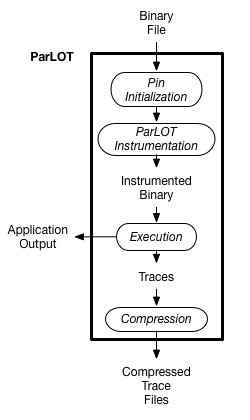
\includegraphics[width=2.2in]{parlot/overview3.png}
\caption{Overview of \parlot}
\label{overview}
\end{figure}


\subsection{Tracing Operation}
\label{subsec:traceOp}

\parlot uses the PIN API as its instrumentation mechanism to gather traces. In particular, it instructs \pin to instrument every thread launch and termination in the application as well as every function entry and exit. The thread-launch instrumentation code initializes the per-thread tracing variables and opens a file into which the trace data from that thread will be written. The thread-termination code finalizes any ongoing compression, flushes out any remaining entries, and closes the trace file. \parlot assigns every static function in each image (main program and all libraries) a unique unsigned 16-bit ID, which it records in a separate file together with the image and function name. This file allows the trace reader to map IDs back to function-name/image pairs.

For every function \emph{entry}, \parlot executes extra code that has access to the thread ID, function ID, and current stack-pointer (SP) value. Based on the SP value, it performs call-stack correction if necessary (see \S\ref{subsec:stack_cor}), adds the new function to a data structure it maintains that holds the call stack (which is separate from the application's runtime stack), and emits the function ID into the trace file via an incremental compression algorithm (see \S\ref{subsec:incr-compr}). All of this is done independently for each thread. Similarly, for every function \emph{exit}, \parlot also executes extra code that has access to the thread ID, function ID, and current SP value. Based on the SP value, it performs call-stack correction if necessary, removes the function from its call-stack data structure, and emits the reserved function ID of zero into the trace file to indicate an exit. As before, this is done via an incremental compression algorithm. We use zero for all exits rather than emitting the function ID and a bit to specify whether it is an entry or exit because using zeros results in more compressible output. This way, half of the values in the trace will be zero.





\subsection{Incremental Compression}
\label{subsec:incr-compr}

\parlot immediately compresses the traced information even before it is written to memory. It does, however, keep a sliding window (circular buffer) of the most recent uncompressed trace events, which is needed by the compressor. It compresses each function ID before the next function ID is known. The conventional approach would be to first record uncompressed function IDs in a buffer and later compress the whole buffer once it fills up. However, this makes the processing time very non-uniform. Whereas almost all function IDs can be recorded very quickly since they just have to be written to the buffer, processing a function ID that happens to fill the buffer takes a long time as it triggers the compression of the entire buffer. This results in sporadic blocking of threads during which time they make no progress towards executing the application code. Initial experiments revealed that such behavior can be detrimental when one thread is polling data from another thread that is currently blocked due to compression. For example, we observed a several order of magnitude increase in entry/exit events of an internal MPI library function when using block-based compression.

To remedy this situation, the compressor must operate incrementally, i.e., each piece of trace data must be compressed when it is generated, without buffering it first, to ensure that there is never a long-latency compression delay. Few existing compression algorithms have been implemented in such a manner because it is more difficult to code up and probably a little slower. Nevertheless, we were able to implement our algorithm (discussed next) in this way so that each trace event is compressed with similar latency.


\subsection{Compression Algorithm}
\label{subsec:compAlg}

We used the CRUSHER framework~\cite{mb-cluster15, mb-space16, mb-sc16, mb-dcc18} to automatically synthesize an effective and fast lossless compression algorithm for our traces. CRUSHER is based on a library of data transformations extracted from various compression algorithms. It combines these transformations in all possible ways to generate algorithm candidates, which it then evaluates on a set of training data. We gathered uncompressed traces from some of the Mantevo miniapps~\cite{mantevo} for this purpose. This evaluation revealed that a particular word-level Lempel-Ziv (LZ) transformation followed by a byte-level Zero-Elimination (ZE) transformation works well. In other words, \parlot 's trace entries, which are two-byte words, are first transformed using LZ. The output is interpreted as a sequence of bytes, which is transformed using ZE for further compression. The output of ZE is written to secondary storage.

LZ implements a variant of the LZ77 algorithm~\cite{LZ}. It uses a 4096-entry hash table to identify the most recent prior occurrence of the current value in the trace. Then it checks whether the three values immediately before that location match the three trace entries just before the current location. If they do not, the current trace entry is emitted and LZ advances to the next entry. If the three values match, LZ counts how many values following the current value match the values following that location. The length of the matching substring is emitted and LZ advances by that many values. Note that all of this is done incrementally. The history of previous trace entries available to LZ for finding matches is maintained in a 64k-entry circular buffer.

ZE emits a bitmap in which each bit represents one input byte. The bits indicate whether the corresponding bytes are zero or not. Following each eight-bit bitmap, ZE emits the non-zero bytes.

As mentioned above, we had to implement the two transformations incrementally to minimize the maximum latency. This required breaking them up into multiple pieces. Depending on the state the compressor is in when the next trace entry needs to be processed, the appropriate piece of code is executed and the state updated. If the LZ code produces an output, which it only does some of the time, then the appropriate piece of the ZE code is executed in a similar manner.


\subsection{PIN and Call-Stack Correction}
\label{subsec:stack_cor}

To be able to decode the trace, i.e., to correctly associate each exit with the function entry it belongs to, our trace reader maintains an identical call-stack data structure. Unfortunately, and as pointed out in the \pin documentation~\cite{pinurl}, it is not always possible to identify all function exits. For example, in optimized code, a function's instructions may be inlined and interleaved with the caller's instructions, making it sometimes infeasible for \pin to identify the exit. As a consequence, we have to ensure that \parlot works correctly even when \pin misses an exit. This is why the SP values are needed.

During tracing, \parlot not only records the function IDs in its call stack but also the associated SP values. This enables it to detect missing exits and to correct the call stack accordingly. Whenever a function is entered, it checks if there is at least one entry in the call stack and, if so, whether its SP value is higher than that of the current SP. If it is lower, we must have missed at least one exit since the runtime stack grows downwards (the SP value decreases with every function entry and increases with every exit). If a missing exit is detected in this manner, \parlot pops the top element from its call stack and emits a zero to indicate a function exit. It repeats this procedure until the stack is empty or its top entry has a sufficiently high SP value. The same call-stack correction technique is applied for every function exit whose SP value is inconsistent. Note that the SP values are only used for this purpose and are not included in the compressed trace.

The result is an internally consistent trace of function entry and exit events, meaning that parsing the trace will yield a correct call stack. This is essential so that the trace can be decoded properly. Moreover, it means that the trace includes exits that truly happened in the application but that were missed by \pin. Note, however, that our call-stack correction is a best-effort approach and may, in rare cases, temporarily not reflect what the application actually did. For example, this can happen for functions that do not create a frame on the runtime stack. When implementing \parlot on top of another DBI framework, call-stack correction may not be needed, resulting in even lower \parlot overhead.


\section{Evaluation Methodology}
\label{sec:ch2_evalmeth}
\subsection{Benchmarks and System}

We performed our evaluations on the MPI-based NAS Parallel Benchmarks (NPB)~\cite{nas}.
%
NPB includes four inputs sizes.
%
To keep the runtimes reasonable, we show results for the class \textit{B} (small-medium) and class \textit{C} (medium-large) inputs.
%

We compiled the NPB codes with the mpicc and mpif77 wrappers of MVAPICH 2.2.1, which are based on icc/ifort 14.0.2 using the prescribed -g and -O1 optimization flags.
%
Quick tests showed that higher optimization levels do not significantly improve the performance.
%

We ran all experiments on Comet at the San Diego Supercomputer Center~\cite{comet}, whose filesystem is NFS and Lustre.
%
Comet has 1944 compute nodes, each of which has dual-socket Intel Xeon E5-2680 v3 processors with a total of 28 cores (14 per socket) and 128 GB of main memory.
%
Note that we only used 16 cores per node as many of the NPB programs require a core count that is a power of two.
%
To study the scaling behavior, we ran experiments on 1, 4, 16 and 64 compute nodes, i.e., on up to 1024 cores.

\subsection{Metrics}

We use the following metrics to quantify and compare the performance of the tracing tools.
%
Unless otherwise noted, all results are based on the median of three identical experiments.
%
\begin{itemize}
\item The \textbf{tracing overhead} is the runtime of the target application when it is being traced divided by the runtime of the same application without tracing.
%
This lower-is-better ratio measures by how much the tracing (and the compression when enabled) slows down the target application.
%
\item The \textbf{tracing bandwidth} is the size of the trace information divided by the application runtime.
%
To make the results easier to compare, we generally list the tracing bandwidth per core, i.e., the tracing bandwidth divided by the number of cores used.
%
This lower-is-better metric is expressed in kilobytes per second (kB/s) per core.
%
It specifies the average needed bandwidth to record the trace data.
%
\item The \textbf{compression ratio} is the size of the uncompressed trace divided by the size of the generated (compressed) trace.
%
This higher-is-better ratio measures the factor by which the compression reduces the trace size.
%
In other words, without compression, the tracing bandwidth would be higher by this factor.
\end{itemize}

\subsection{Tracing Tools}
\label{sec:tracing-tools}

We compare our \parlot tool, implemented on top of \pin 3.5, with \callgrind 3.13.
%
\parlot was compiled with gcc 4.9.2 using \pin 's make system and \callgrind with Valgrind's make system.
%
We created the following versions of \parlot to evaluate different aspects of its design.

% ORIGINAL TABLE
\iffalse
\begin{table}[]
\caption{Overhead added by each tool. Last column is the geometric mean}
\label{comet_sd_pMpAcg_BC_itn_p3.5}\begin{center}
\npdecimalsign{.}
\nprounddigits{1}
\begin{tabular}{lrrrrrrrrr}
\hline
                &   bt &   cg &    ep &    ft &   is &   lu &   mg &   sp &   GM \\
\hline
 pinMain.B.1    & 1.55 & 1.82 &  2.62 &  2.11 & 2.47 & 1.31 & 2.53 & 1.33 & 1.90 \\
 pinMain.B.4    & 1.76 & 1.85 &  1.89 &  1.74 & 1.78 & 1.77 & 1.52 & 1.73 & 1.75 \\
 pinMain.B.16   & 2.15 & 2.58 &  1.99 &  1.89 & 1.78 & 2.73 & 2.43 & 2.15 & 2.19 \\
 pinMain.B.64   & 2.10 & 2.17 &  2.39 &  1.96 & 4.31 & 4.39 & 1.97 & 2.07 & 2.52 \\
 AVG            & 1.89 & 2.10 &  2.22 &  1.92 & 2.58 & 2.55 & 2.11 & 1.82 & 2.09 \\
 pinAll.B.1     & 1.84 & 2.73 &  4.18 &  2.78 & 4.22 & 1.73 & 4.75 & 1.72 & 2.77 \\
 pinAll.B.4     & 2.57 & 3.06 &  3.41 &  2.77 & 2.96 & 2.76 & 2.79 & 2.66 & 2.86 \\
 pinAll.B.16    & 3.52 & 4.20 &  3.39 &  2.94 & 2.83 & 4.30 & 4.46 & 3.65 & 3.62 \\
 pinAll.B.64    & 3.14 & 3.26 &  3.83 &  3.02 & 5.44 & 4.65 & 3.17 & 3.31 & 3.65 \\
 AVG            & 2.77 & 3.31 &  3.70 &  2.88 & 3.86 & 3.36 & 3.79 & 2.83 & 3.23 \\
 callgrind.B.1  & 8.62 & 5.96 &  8.92 & 10.14 & 2.52 & 7.54 & 3.27 & 6.61 & 6.10 \\
 callgrind.B.4  & 6.02 & 3.60 &  2.90 &  3.50 & 1.46 & 5.18 & 1.24 & 5.78 & 3.23 \\
 callgrind.B.16 & 4.28 & 3.26 &  2.24 &  2.17 & 1.70 & 4.62 & 1.81 & 4.34 & 2.84 \\
 callgrind.B.64 & 2.26 & 2.03 &  1.66 &  2.05 & 4.07 & 3.97 & 1.47 & 2.46 & 2.34 \\
 AVG            & 5.29 & 3.71 &  3.93 &  4.46 & 2.44 & 5.33 & 1.95 & 4.80 & 3.63 \\
 pinMain.C.1    & 1.41 & 1.29 &  2.51 &  1.89 & 2.29 & 1.12 & 1.74 & 1.10 & 1.60 \\
 pinMain.C.4    & 1.58 & 1.73 &  1.75 &  1.62 & 1.68 & 1.33 & 1.81 & 1.35 & 1.60 \\
 pinMain.C.16   & 1.82 & 2.38 &  2.46 &  1.51 & 1.80 & 2.18 & 2.36 & 1.80 & 2.01 \\
 pinMain.C.64   & 2.23 & 2.74 &  2.39 &  1.59 & 4.46 & 3.42 & 2.43 & 2.24 & 2.57 \\
 AVG            & 1.76 & 2.04 &  2.28 &  1.65 & 2.56 & 2.01 & 2.08 & 1.62 & 1.94 \\
 pinAll.C.1     & 1.47 & 1.55 &  3.17 &  1.97 & 2.82 & 1.23 & 2.52 & 1.19 & 1.87 \\
 pinAll.C.4     & 1.89 & 2.42 &  2.56 &  2.06 & 2.56 & 1.70 & 3.08 & 1.71 & 2.20 \\
 pinAll.C.16    & 2.69 & 3.47 &  4.07 &  2.14 & 2.80 & 3.18 & 3.98 & 2.54 & 3.04 \\
 pinAll.C.64    & 3.61 & 4.13 &  4.21 &  2.22 & 5.47 & 4.43 & 4.23 & 3.02 & 3.80 \\
 AVG            & 2.42 & 2.89 &  3.50 &  2.10 & 3.41 & 2.63 & 3.45 & 2.11 & 2.73 \\
 callgrind.C.1  & 8.50 & 4.44 & 13.18 & 13.13 & 3.32 & 7.90 & 5.91 & 5.14 & 6.91 \\
 callgrind.C.4  & 8.66 & 4.46 &  4.76 &  6.37 & 1.65 & 6.38 & 2.75 & 6.34 & 4.64 \\
 callgrind.C.16 & 6.86 & 3.91 &  3.11 &  2.76 & 1.79 & 6.40 & 2.14 & 6.09 & 3.69 \\
 callgrind.C.64 & 4.37 & 3.46 &  2.13 &  2.50 & 4.24 & 5.24 & 2.08 & 3.81 & 3.30 \\
 AVG            & 7.10 & 4.07 &  5.79 &  6.19 & 2.75 & 6.48 & 3.22 & 5.34 & 4.63 \\
\hline
\end{tabular}
\npnoround
\end{center}
\end{table}
\fi



\iftrue

\begin{table}[!b]
\caption{Overhead added by each tool}
\label{comet_sd_pMpAcg_BC_itn_p3.5}\begin{center}
\npdecimalsign{.}
\nprounddigits{1}
\scalebox{0.80}{
\begin{tabular}{|c|c|c|n{2}{1}n{2}{1}n{2}{1}n{2}{1}n{2}{1}n{2}{1}n{2}{1}n{2}{1}|n{2}{1}|}
\hline
Input & Tool & \# Nodes  & \multicolumn{1}{c}{bt} & \multicolumn{1}{c}{cg} & \multicolumn{1}{c}{ep} & \multicolumn{1}{c}{ft} & \multicolumn{1}{c}{is} & \multicolumn{1}{c}{lu} & \multicolumn{1}{c}{mg} & \multicolumn{1}{c|}{sp} & \multicolumn{1}{c|}{GM} \\ \hline
\multirow{15}{*}{B} & \multirow{5}{*}{\parlotm} & 1 & 1.55 & 1.82 &  2.62 &  2.11 & 2.47 & 1.31 & 2.53 & 1.33 & 1.90 \\
 &  & 4  & 1.76 & 1.85 &  1.89 &  1.74 & 1.78 & 1.77 & 1.52 & 1.73 & 1.75 \\
 &  & 16  & 2.15 & 2.58 &  1.99 &  1.89 & 1.78 & 2.73 & 2.43 & 2.15 & 2.19 \\
 &  & 64  & 2.10 & 2.17 &  2.39 &  1.96 & 4.31 & 4.39 & 1.97 & 2.07 & 2.52 \\ \cline{3-12}
 &  & AVG & 1.89 & 2.10 &  2.22 &  1.92 & 2.58 & 2.55 & 2.11 & 1.82 & {\boldmath}2.09 \\ \cline{2-12}
 & \multirow{5}{*}{\parlota} & 1 & 1.84 & 2.73 &  4.18 &  2.78 & 4.22 & 1.73 & 4.75 & 1.72 & 2.77 \\
 & & 4     & 2.57 & 3.06 &  3.41 &  2.77 & 2.96 & 2.76 & 2.79 & 2.66 & 2.86 \\
 & & 16    & 3.52 & 4.20 &  3.39 &  2.94 & 2.83 & 4.30 & 4.46 & 3.65 & 3.62 \\
 & & 64    & 3.14 & 3.26 &  3.83 &  3.02 & 5.44 & 4.65 & 3.17 & 3.31 & 3.65 \\ \cline{3-12}
 & & AVG   & 2.77 & 3.31 &  3.70 &  2.88 & 3.86 & 3.36 & 3.79 & 2.83 & {\boldmath}3.23 \\ \cline{2-12}
 & \multirow{5}{*}{\callgrind}  & 1  & 8.62 & 5.96 &  8.92 & 10.14 & 2.52 & 7.54 & 3.27 & 6.61 & 6.10 \\
 & & 4   & 6.02 & 3.60 &  2.90 &  3.50 & 1.46 & 5.18 & 1.24 & 5.78 & 3.23 \\
 & & 16  & 4.28 & 3.26 &  2.24 &  2.17 & 1.70 & 4.62 & 1.81 & 4.34 & 2.84 \\
 & & 64  & 2.26 & 2.03 &  1.66 &  2.05 & 4.07 & 3.97 & 1.47 & 2.46 & 2.34 \\ \cline{3-12}
 & & AVG & 5.29 & 3.71 &  3.93 &  4.46 & 2.44 & 5.33 & 1.95 & 4.80 & {\boldmath}3.63 \\ \hline
 \multirow{15}{*}{C} & \multirow{5}{*}{\parlotm} & 1  & 1.41 & 1.29 &  2.51 &  1.89 & 2.29 & 1.12 & 1.74 & 1.10 & 1.60 \\
 & & 4   & 1.58 & 1.73 &  1.75 &  1.62 & 1.68 & 1.33 & 1.81 & 1.35 & 1.60 \\
 & & 16  & 1.82 & 2.38 &  2.46 &  1.51 & 1.80 & 2.18 & 2.36 & 1.80 & 2.01 \\
 & & 64  & 2.23 & 2.74 &  2.39 &  1.59 & 4.46 & 3.42 & 2.43 & 2.24 & 2.57 \\ \cline{3-12}
 & & AVG & 1.76 & 2.04 &  2.28 &  1.65 & 2.56 & 2.01 & 2.08 & 1.62 & {\boldmath}1.94 \\ \cline{2-12}
 & \multirow{5}{*}{\parlota} & 1 & 1.47 & 1.55 &  3.17 &  1.97 & 2.82 & 1.23 & 2.52 & 1.19 & 1.87 \\
 & & 4   & 1.89 & 2.42 &  2.56 &  2.06 & 2.56 & 1.70 & 3.08 & 1.71 & 2.20 \\
 & & 16  & 2.69 & 3.47 &  4.07 &  2.14 & 2.80 & 3.18 & 3.98 & 2.54 & 3.04 \\
 & & 64  & 3.61 & 4.13 &  4.21 &  2.22 & 5.47 & 4.43 & 4.23 & 3.02 & 3.80 \\ \cline{3-12}
 & & AVG & 2.42 & 2.89 &  3.50 &  2.10 & 3.41 & 2.63 & 3.45 & 2.11 & {\boldmath}2.73 \\ \cline{2-12}
 & \multirow{5}{*}{\callgrind} & 1 & 8.50 & 4.44 & 13.18 & 13.13 & 3.32 & 7.90 & 5.91 & 5.14 & 6.91 \\
 & & 4   & 8.66 & 4.46 &  4.76 &  6.37 & 1.65 & 6.38 & 2.75 & 6.34 & 4.64 \\
 & & 16  & 6.86 & 3.91 &  3.11 &  2.76 & 1.79 & 6.40 & 2.14 & 6.09 & 3.69 \\
 & & 64  & 4.37 & 3.46 &  2.13 &  2.50 & 4.24 & 5.24 & 2.08 & 3.81 & 3.30 \\ \cline{3-12}
 & & AVG & 7.10 & 4.07 &  5.79 &  6.19 & 2.75 & 6.48 & 3.22 & 5.34 & {\boldmath}4.63 \\ \hline
\end{tabular}}
\npnoround
\end{center}
\end{table}

\fi



\begin{itemize}
\item \textbf{\parlotm} is the normal \parlot tool configured to only collect function-call traces from the main image of the application.
\item \textbf{\parlota} is the normal \parlot tool configured to collect function-call traces from all images of the application, including library function calls.
\item \textbf{\pininit} is a crippled version of \parlot from which the tracing code has been removed.
%
The purpose of \pininit is to see how much of the overhead is due to \pin.
\item \textbf{\parlotnc} is the normal \parlot tool but with compression disabled.
%
It writes out the captured data in uncompressed form.
%
The purpose of \parlotnc is to show the performance impact of the compression.
\end{itemize}

It proved surprisingly difficult to find a tool that is similar to \parlot because there appear to be no other tools that generate whole program call traces.
%
In the end, we settled on \callgrind as the most similar tool we could find and used it for our comparisons.
%
\callgrind is based on the Valgrind DBI tool.
%
It collects function-call graphs combined with performance data to show the user what portion of the execution time has been spent in each function.

%%%%%%%%%%%%%%%%%%%%%%%%%%%%%%%%%
% FROM RESULTS - average overhead
%%%%%%%%%%%%%%%%%%%%%%%%%%%%%%%%%

Each \callgrind trace file contains a sequence of function names (or their code) plus numerical data for each function on its caller-callee relationship with other functions.
%
Moreover, it contains cost information for each function in terms of how many machine instructions it read.
%
This information is collected using hardware performance counters.
%
The format of the file is plain ASCII text.
%
Interestingly, all numerical values are expressed relative to previous values, i.e., they are delta (or difference) encoded.
%
This simple form of compression is enabled by default in \callgrind.


\begin{figure}[b]
\centering
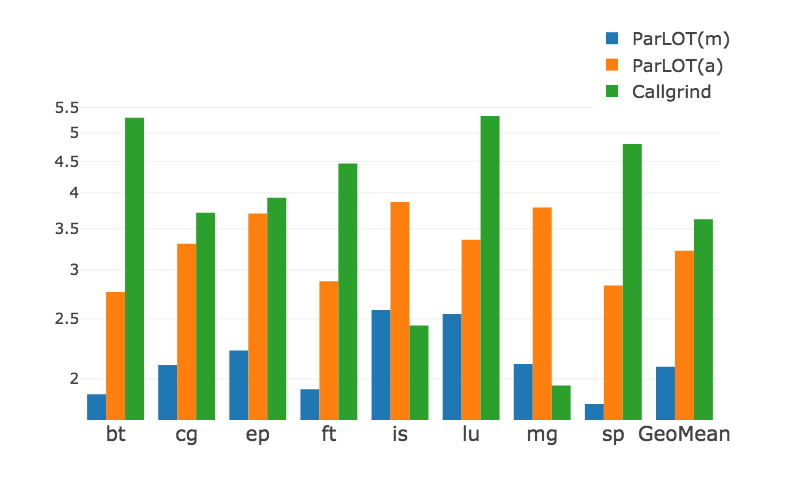
\includegraphics[width=.75\textwidth]{parlot/figs.comet.newMed/comet_chartAvg_sd_B_p3_5.png}
\caption{Average tracing overhead on the NPB applications - Input B}
\label{comet_chartAvg_sd_B_p3_5}
\end{figure}

\begin{figure}[b]
\centering
%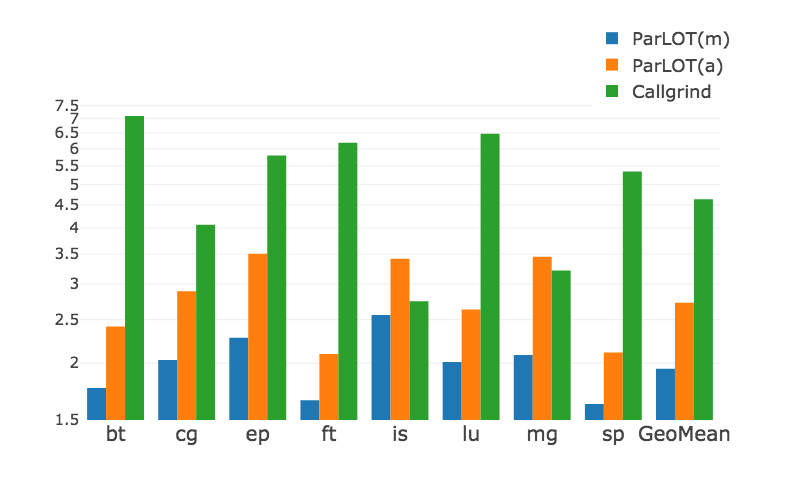
\includegraphics[width=3.4in,height=1.9in]{parlot/figs.comet.newMed/comet_chartAvg_sd_C_p3_5.png}
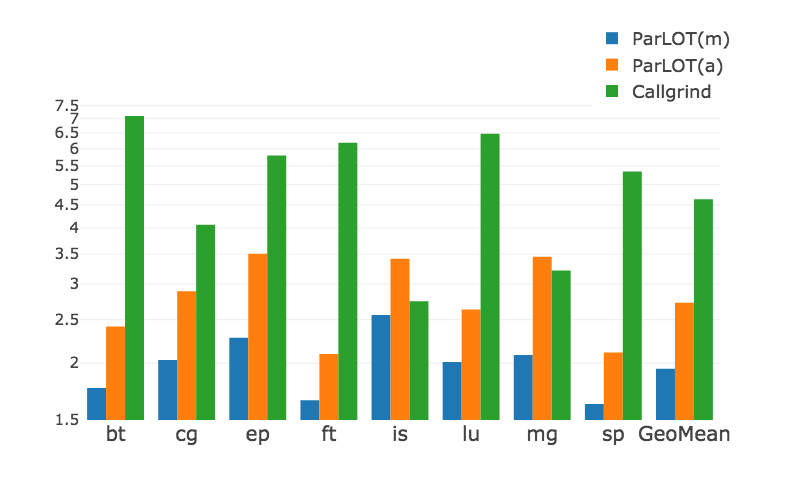
\includegraphics[width=.75\textwidth]{parlot/figs.comet.newMed/comet_chartAvg_sd_C_p3_5.png}
\caption{ Average tracing overhead on the NPB applications - Input C}
\label{comet_chartAvg_sd_C_p3_5}
\end{figure}


We believe the information traced by \callgrind is reasonably similar to the information traced by \parlotm.
%
Whereas \callgrind 's traces include performance data that \parlot does not capture, \parlot records the whole-program call trace, which \callgrind does not capture.
%
The full function-call trace is a strict superset of the call-graph information that \callgrind records because the call graph can be extracted from the function-call trace but not vice versa.
%
In particular, \callgrind cannot recreate the order of the function calls a thread made whereas \parlot can.


\section{Results}
\label{sec:ch2_results}
%%%%%%%%%%%%%%%%%%%%%%%%%%%%%%%%%%%%%
% Tracing Overhead
%%%%%%%%%%%%%%%%%%%%%%%%%%%%%%%%%%%%%

\subsection{Tracing Overhead}
\label{subsec:lowtoh}
\iffalse

\begin{table*}[]
\caption{Req BW}
\label{comet_bw_pMpAcg_BC_itn_p3.5}\begin{center}
\begin{tabular}{lrrrrrrrrr}
\hline
                &    bt &     cg &    ep &    ft &    is &     lu &    mg &     sp &    GM \\
\hline
 pinMain.B.1    &  4.72 &  21.86 &  3.83 &  1.52 &  0.79 &   2.39 &  5.62 &   5.36 &  3.69 \\
 pinMain.B.4    & 14.28 &  41.08 &  1.89 &  3.48 &  2.24 &  21.48 &  6.45 &  15.85 &  8.12 \\
 pinMain.B.16   & 14.31 &  46.59 &  1.45 &  4.86 &  3.40 &  31.79 &  6.53 &  18.55 &  9.41 \\
 pinMain.B.64   & 18.56 &  43.59 &  1.25 &  4.56 &  4.49 &  27.07 &  5.63 &  29.62 &  9.92 \\
 AVG            & 12.97 &  38.28 &  2.10 &  3.60 &  2.73 &  20.68 &  6.06 &  17.35 &  7.79 \\
 pinAll.B.1     & 48.71 &  89.39 & 47.23 & 45.63 & 59.98 &  53.62 & 60.81 &  54.33 & 56.21 \\
 pinAll.B.4     & 61.84 & 101.23 & 45.21 & 55.12 & 53.20 &  71.09 & 54.85 &  73.62 & 62.68 \\
 pinAll.B.16    & 73.95 & 116.87 & 47.37 & 48.88 & 47.79 & 100.91 & 55.80 &  84.61 & 67.97 \\
 pinAll.B.64    & 81.80 & 110.15 & 44.16 & 47.98 & 37.84 & 100.26 & 52.67 &  99.90 & 66.47 \\
 AVG            & 66.58 & 104.41 & 45.99 & 49.40 & 49.70 &  81.47 & 56.03 &  78.12 & 63.33 \\
 callgrind.B.1  &  1.57 &   7.69 &  7.39 &  4.56 & 39.49 &   2.61 & 34.41 &   2.71 &  6.67 \\
 callgrind.B.4  &  6.51 &  16.01 & 22.10 & 15.65 & 45.46 &   8.63 & 45.47 &   7.78 & 16.31 \\
 callgrind.B.16 & 17.20 &  24.62 & 37.42 & 23.84 & 29.87 &  16.23 & 51.49 &  15.81 & 24.93 \\
 callgrind.B.64 & 26.82 &  27.65 & 45.93 & 25.14 & 11.04 &  17.75 & 45.27 &  20.20 & 25.02 \\
 AVG            & 13.03 &  18.99 & 28.21 & 17.30 & 31.47 &  11.30 & 44.16 &  11.62 & 18.23 \\
 pinMain.C.1    &  1.82 &  16.96 &  5.15 &  1.16 &  0.69 &   0.77 &  3.56 &   1.40 &  2.17 \\
 pinMain.C.4    &  7.53 &  44.87 &  3.00 &  2.50 &  2.12 &  20.13 &  7.08 &  13.74 &  7.55 \\
 pinMain.C.16   & 16.30 &  55.04 &  1.84 &  6.10 &  3.35 &  34.09 &  7.24 &  20.68 & 10.70 \\
 pinMain.C.64   & 17.45 &  61.43 &  1.30 &  5.93 &  4.42 &  38.28 &  5.62 &  26.09 & 10.94 \\
 AVG            & 10.77 &  44.58 &  2.82 &  3.92 &  2.65 &  23.32 &  5.88 &  15.48 &  7.84 \\
 pinAll.C.1     & 17.80 &  53.37 & 26.34 & 20.89 & 48.31 &  25.31 & 52.61 &  19.46 & 29.99 \\
 pinAll.C.4     & 51.78 &  95.84 & 36.80 & 43.82 & 51.40 &  58.39 & 54.18 &  65.77 & 55.15 \\
 pinAll.C.16    & 75.38 & 121.03 & 44.29 & 61.39 & 46.90 & 101.05 & 56.49 & 101.32 & 71.37 \\
 pinAll.C.64    & 80.63 & 135.19 & 43.49 & 46.28 & 37.09 & 117.87 & 54.05 &  99.02 & 68.99 \\
 AVG            & 56.40 & 101.36 & 37.73 & 43.09 & 45.93 &  75.66 & 54.33 &  71.39 & 56.38 \\
 callgrind.C.1  &  0.40 &   3.09 &  1.96 &  1.05 & 14.60 &   0.70 &  6.96 &   0.75 &  1.85 \\
 callgrind.C.4  &  1.78 &   8.87 &  7.74 &  4.48 & 31.74 &   2.82 & 21.03 &   2.78 &  6.41 \\
 callgrind.C.16 &  6.01 &  15.82 & 22.86 & 10.75 & 26.50 &   7.45 & 39.05 &   6.96 & 13.72 \\
 callgrind.C.64 & 14.32 &  19.56 & 35.75 & 12.17 & 11.07 &  11.86 & 40.69 &  12.83 & 17.39 \\
 AVG            &  5.63 &  11.84 & 17.08 &  7.11 & 20.98 &   5.71 & 26.93 &   5.83 &  9.84 \\
\hline
\end{tabular}
\end{center}
\end{table*}

\fi


\iftrue

\begin{table*}[]
\caption{ Required bandwidth per core (kB/s) }
\label{comet_bw_pMpAcg_BC_itn_p3.5}\begin{center}
\npdecimalsign{.}
\nprounddigits{1}
\scalebox{0.90}{
\begin{tabular}{|c|c|c|n{3}{1}n{3}{1}n{3}{1}n{3}{1}n{3}{1}n{3}{1}n{3}{1}n{3}{1}|n{3}{1}|}
\hline
Input & Tool & \# Nodes  & \multicolumn{1}{c}{bt} & \multicolumn{1}{c}{cg} & \multicolumn{1}{c}{ep} & \multicolumn{1}{c}{ft} & \multicolumn{1}{c}{is} & \multicolumn{1}{c}{lu} & \multicolumn{1}{c}{mg} & \multicolumn{1}{c|}{sp} & \multicolumn{1}{c|}{GM} \\ \hline
\multirow{15}{*}{B} & \multirow{5}{*}{\parlotm} & 1 &  4.72 &  21.86 &  3.83 &  1.52 &  0.79 &   2.39 &  5.62 &   5.36 &  3.69 \\
 & & 4                                               & 14.28 &  41.08 &  1.89 &  3.48 &  2.24 &  21.48 &  6.45 &  15.85 &  8.12 \\
 & & 16                                              & 14.31 &  46.59 &  1.45 &  4.86 &  3.40 &  31.79 &  6.53 &  18.55 &  9.41 \\
 & & 64                                              & 18.56 &  43.59 &  1.25 &  4.56 &  4.49 &  27.07 &  5.63 &  29.62 &  9.92 \\ \cline{3-12} 
 & & AVG                                             & 12.97 &  38.28 &  2.10 &  3.60 &  2.73 &  20.68 &  6.06 &  17.35 &  {\boldmath}7.79  \\ \cline{2-12} 
 & \multirow{5}{*}{\parlota} & 1 & 48.71 &  89.39 & 47.23 & 45.63 & 59.98 &  53.62 & 60.81 &  54.33 & 56.21 \\
 & & 4                            & 61.84 & 101.23 & 45.21 & 55.12 & 53.20 &  71.09 & 54.85 &  73.62 & 62.68 \\
 & & 16                           & 73.95 & 116.87 & 47.37 & 48.88 & 47.79 & 100.91 & 55.80 &  84.61 & 67.97 \\
 & & 64                           & 81.80 & 110.15 & 44.16 & 47.98 & 37.84 & 100.26 & 52.67 &  99.90 & 66.47 \\ \cline{3-12} 
 & & AVG                          & 66.58 & 104.41 & 45.99 & 49.40 & 49.70 &  81.47 & 56.03 &  78.12 & {\boldmath}63.33 \\ \cline{2-12} 
 & \multirow{5}{*}{\callgrind}  & 1  &  1.57 &   7.69 &  7.39 &  4.56 & 39.49 &   2.61 & 34.41 &   2.71 &  6.67  \\
 & & 4                              &  6.51 &  16.01 & 22.10 & 15.65 & 45.46 &   8.63 & 45.47 &   7.78 & 16.31  \\
 & & 16                             & 17.20 &  24.62 & 37.42 & 23.84 & 29.87 &  16.23 & 51.49 &  15.81 & 24.93  \\
 & & 64                             & 26.82 &  27.65 & 45.93 & 25.14 & 11.04 &  17.75 & 45.27 &  20.20 & 25.02  \\ \cline{3-12} 
 & & AVG                            & 13.03 &  18.99 & 28.21 & 17.30 & 31.47 &  11.30 & 44.16 &  11.62 & {\boldmath}18.23  \\ \hline
 \multirow{15}{*}{C} & \multirow{5}{*}{\parlotm} & 1  &  1.82 &  16.96 &  5.15 &  1.16 &  0.69 &   0.77 &  3.56 &   1.40 &  2.17  \\
 & & 4                                                 &  7.53 &  44.87 &  3.00 &  2.50 &  2.12 &  20.13 &  7.08 &  13.74 &  7.55  \\
 & & 16                                                & 16.30 &  55.04 &  1.84 &  6.10 &  3.35 &  34.09 &  7.24 &  20.68 & 10.70  \\
 & & 64                                                & 17.45 &  61.43 &  1.30 &  5.93 &  4.42 &  38.28 &  5.62 &  26.09 & 10.94  \\ \cline{3-12} 
 & & AVG                                               & 10.77 &  44.58 &  2.82 &  3.92 &  2.65 &  23.32 &  5.88 &  15.48 &  {\boldmath}7.84  \\ \cline{2-12} 
 & \multirow{5}{*}{\parlota} & 1 & 17.80 &  53.37 & 26.34 & 20.89 & 48.31 &  25.31 & 52.61 &  19.46 & 29.99 \\
 & & 4                            & 51.78 &  95.84 & 36.80 & 43.82 & 51.40 &  58.39 & 54.18 &  65.77 & 55.15 \\
 & & 16                           & 75.38 & 121.03 & 44.29 & 61.39 & 46.90 & 101.05 & 56.49 & 101.32 & 71.37 \\
 & & 64                           & 80.63 & 135.19 & 43.49 & 46.28 & 37.09 & 117.87 & 54.05 &  99.02 & 68.99 \\ \cline{3-12}
 & & AVG                          & 56.40 & 101.36 & 37.73 & 43.09 & 45.93 &  75.66 & 54.33 &  71.39 & {\boldmath}56.38  \\ \cline{2-12} 
 & \multirow{5}{*}{\callgrind} & 1 &  0.40 &   3.09 &  1.96 &  1.05 & 14.60 &   0.70 &  6.96 &   0.75 &  1.85  \\
 & & 4                            &  1.78 &   8.87 &  7.74 &  4.48 & 31.74 &   2.82 & 21.03 &   2.78 &  6.41  \\
 & & 16                           &  6.01 &  15.82 & 22.86 & 10.75 & 26.50 &   7.45 & 39.05 &   6.96 & 13.72  \\
 & & 64                           & 14.32 &  19.56 & 35.75 & 12.17 & 11.07 &  11.86 & 40.69 &  12.83 & 17.39  \\ \cline{3-12}
 & & AVG                          &  5.63 &  11.84 & 17.08 &  7.11 & 20.98 &   5.71 & 26.93 &   5.83 &  {\boldmath}9.84  \\ \hline
\end{tabular}}
\end{center}
\end{table*}

\fi


%%%%%%%%%%%%%%%%%%%%%%%%%%%%%%%%%
% FROM RESULTS - average bandwidth
%%%%%%%%%%%%%%%%%%%%%%%%%%%%%%%%%
\begin{figure}[t]
\centering
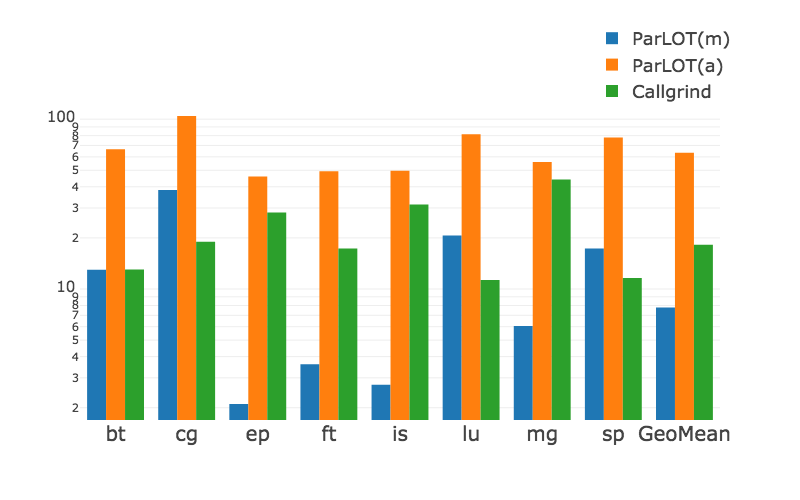
\includegraphics[width=3.4in,height=1.9in]{parlot/figs.comet.newMed/comet_chartAvg_bw_B_p3_5.png}
\caption{  Average required bandwidth per core (kB/s) on the NPB applications - Input B}
\label{comet_chartAvg_bw_B_p3_5}
\end{figure}

\begin{figure}[t]
\centering
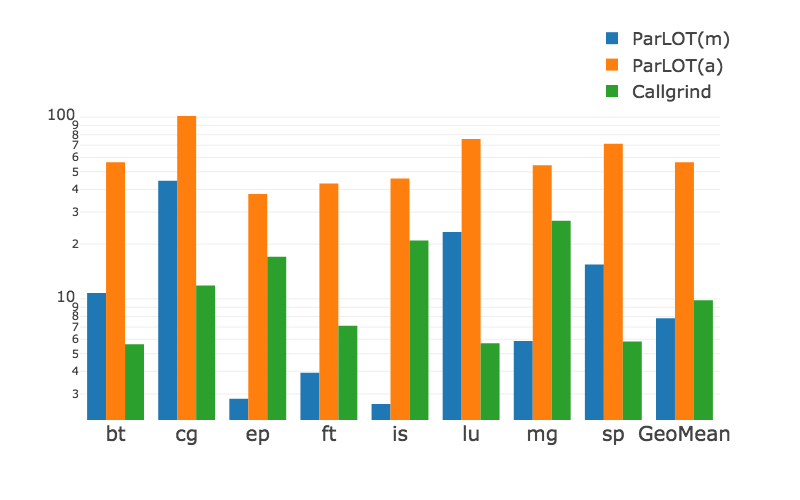
\includegraphics[width=3.4in,height=1.9in]{parlot/figs.comet.newMed/comet_chartAvg_bw_C_p3_5.png}
\caption{ Average required bandwidth per core (kB/s) on the NPB applications - Input C}
\label{comet_chartAvg_bw_C_p3_5}
\end{figure}

%%%%%%%%%%%%%%%%%%%%%%%%%%%%%%%%%
% ENDDDD
%%%%%%%%%%%%%%%%%%%%%%%%%%%%%%%%%

Table \ref{comet_sd_pMpAcg_BC_itn_p3.5} shows the tracing overhead of \parlotm, \parlota, and \callgrind on each application of the NPB benchmark suite for different node counts. The last column of the table lists the geometric mean over all eight programs. The AVG rows show the average over the four node counts.


On average, both \parlotm and \parlota outperform \callgrind. The bolded numbers in Table \ref{comet_sd_pMpAcg_BC_itn_p3.5} for input C show that the average overhead is 1.94 for \parlotm, 2.73 for \parlota, and 4.63 for \callgrind. Figures \ref{comet_chartAvg_sd_B_p3_5} and \ref{comet_chartAvg_sd_C_p3_5} show these results in visual form.


The key takeaway point is that the overhead of \parlot is roughly a factor of two to three, which we believe users may be willing to accept, for example, if it helps them debug their applications. This is promising especially when considering how detailed the collected trace information is and that most of the overhead is due to \pin (see \S\ref{subsec:pinit}). Note that \parlot 's overhead is typically lower than that of \callgrind, which collects less information.

The overhead of \parlot increases as we scale the applications to more compute nodes. However, the increase is quite small. Going from 16 to 1024 cores, a 64-fold increase in parallelism, only increases the average overhead by between 1.3- and 2.1-fold. In contrast, \callgrind 's overhead decreases with increasing node count, making it more scalable. Having said that, \callgrind 's overhead is larger for the C inputs whereas \parlot 's overhead is larger for the smaller B inputs. In other words, \parlot scales better to larger inputs than \callgrind.

\parlot 's scaling behavior can be explained by correlating it with the expected function-call frequency. When distributing a fixed problem size over more cores, each core receives less work. As a consequence, less time is spent in the functions that process the work, resulting in more function calls per time unit, which causes more work for \parlot. In contrast, when distributing a larger problem size over the same number of cores, each core receives more work. Hence, more time is spent in the functions that process the work, resulting in fewer function calls per time unit, which causes less work for \parlot and therefore less tracing overhead. Hence, we believe \parlot 's overhead to be even lower on long-running inputs, which is where our tracing technique is needed the most.


In summary, \parlot 's overhead is in the single digits for all evaluated applications and configurations, including for 1024-core runs. It appears to scale reasonably to larger node counts and well to larger problem sizes.

\subsection{Required Bandwidth}
\label{subsec:lowbw}

Table \ref{comet_bw_pMpAcg_BC_itn_p3.5}, Fig.  \ref{comet_chartAvg_bw_B_p3_5} and Fig. \ref{comet_chartAvg_bw_C_p3_5} show how much trace bandwidth each tool
requires
during the application execution.
%
On average, \parlotm requires less bandwidth than
\callgrind, especially for smaller inputs.
%
\parlota's bandwidth is much higher as it collects call information from all
images and not just the main image like \parlotm does.

We see that the required bandwidth for different input sizes of the NPB applications are almost equal in \parlot. According to the NPB documentation, the number of iterations for inputs B and C are the same for all applications. They only differ in the number of elements or the grid size. It is clear that the required bandwidth of \parlot is independent of the problem size, unlike \callgrind, where the input size has a linear impact on the results.

%
%%%%%%%%%%%%%%%%%%%%%%%%%%%%%%%%%
% FROM RESULTS - average compression ratio
%%%%%%%%%%%%%%%%%%%%%%%%%%%%%%%%%
\begin{figure}[t]
\centering
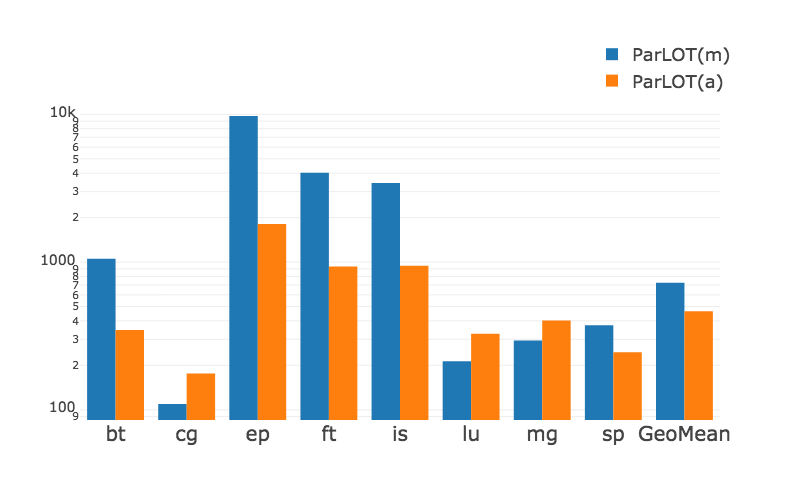
\includegraphics[width=3.2in,height=1.9in]{parlot/figs.comet.newMed/comet_chartAvg_cr_B_p3_5.png}
\caption{ Average compression ratio of \parlot on the NPB applications - Input B}
\label{comet_chartAvg_cr_B_p3_5}
\end{figure}

\begin{figure}[t]
\centering
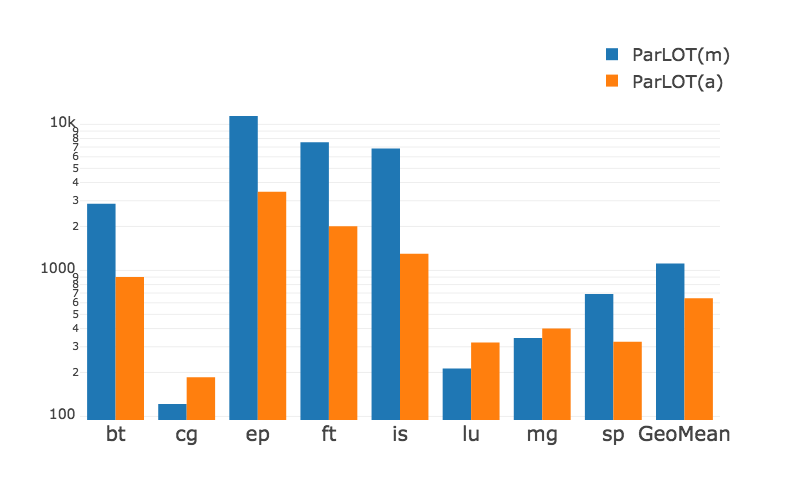
\includegraphics[width=3.2in,height=1.9in]{parlot/figs.comet.newMed/comet_chartAvg_cr_C_p3_5.png}
\caption{ Average compression ratio of \parlot on the NPB applications - Input C}
\label{comet_chartAvg_cr_C_p3_5}
\end{figure}
%%%%%%%%%%%%%%%%%%%%%%%%%%%%%%%%%
% ENDDDD
%%%%%%%%%%%%%%%%%%%%%%%%%%%%%%%%%



\iffalse
\begin{table}[]
\caption{Compression Ratio}
\label{comet_cr_pMpA_BC_itn_p3.5}\begin{center}
\begin{tabular}{lrrrrrrrrr}
\hline
              &      bt &     cg &       ep &       ft &       is &     lu &     mg &      sp &      GM \\
\hline
 pinMain.B.1  & 3035.93 &  94.35 & 12456.18 & 12173.49 &  9718.38 & 167.72 &  99.08 &  878.27 & 1255.17 \\
 pinMain.B.4  &  586.64 &  82.48 & 10368.41 &  1737.09 &   909.20 & 140.29 & 254.95 &  338.16 &  559.36 \\
 pinMain.B.16 &  346.66 & 113.28 &  8563.85 &  1077.35 &  1200.57 & 178.98 & 387.63 &  123.02 &  496.83 \\
 pinMain.B.64 &  252.24 & 147.78 &  7611.04 &  1122.62 &  1907.95 & 366.80 & 437.31 &  152.91 &  591.11 \\
 AVG          & 1055.37 & 109.47 &  9749.87 &  4027.64 &  3434.03 & 213.45 & 294.74 &  373.09 &  725.62 \\
 pinAll.B.1   &  514.51 & 137.41 &  3335.77 &  1226.74 &   543.18 & 314.63 & 260.87 &  303.88 &  500.21 \\
 pinAll.B.4   &  315.71 & 137.21 &  1266.92 &   436.15 &   316.16 & 287.25 & 329.57 &  199.66 &  330.70 \\
 pinAll.B.16  &  226.86 & 181.58 &  1246.66 &  1026.53 &   927.09 & 299.30 & 469.29 &  171.52 &  430.39 \\
 pinAll.B.64  &  329.23 & 247.30 &  1394.07 &  1043.94 &  1984.62 & 410.32 & 548.47 &  307.16 &  597.55 \\
 AVG          &  346.58 & 175.88 &  1810.86 &   933.34 &   942.76 & 327.88 & 402.05 &  245.56 &  464.71 \\
 pinMain.C.1  & 8618.95 & 111.16 & 13067.96 & 21335.57 & 21856.49 & 350.03 & 247.44 & 1977.43 & 2371.35 \\
 pinMain.C.4  & 1910.64 & 110.45 & 12418.66 &  6520.34 &  2256.56 & 112.77 & 267.98 &  472.68 &  928.16 \\
 pinMain.C.16 &  580.79 & 133.24 & 11017.36 &  1239.31 &  1347.88 & 164.47 & 396.86 &  143.13 &  582.78 \\
 pinMain.C.64 &  322.83 & 131.92 &  9154.99 &  1065.12 &  1896.25 & 223.69 & 465.74 &  168.89 &  585.74 \\
 AVG          & 2858.30 & 121.69 & 11414.74 &  7540.09 &  6839.30 & 212.74 & 344.50 &  690.53 & 1117.01 \\
 pinAll.C.1   & 2579.37 & 181.76 &  7376.96 &  5143.08 &  1520.42 & 408.21 & 314.77 &  650.73 & 1107.37 \\
 pinAll.C.4   &  448.61 & 161.32 &  3194.58 &  1062.94 &   527.34 & 274.70 & 319.35 &  237.43 &  477.42 \\
 pinAll.C.16  &  285.05 & 185.74 &  1765.49 &   588.86 &  1106.34 & 273.63 & 467.35 &  141.69 &  426.92 \\
 pinAll.C.64  &  290.00 & 214.68 &  1512.89 &  1237.30 &  2038.72 & 329.04 & 496.21 &  270.83 &  565.82 \\
 AVG          &  900.76 & 185.88 &  3462.48 &  2008.05 &  1298.21 & 321.39 & 399.42 &  325.17 &  644.38 \\
\hline
\end{tabular}
\end{center}
\end{table}

\fi


\iftrue

\begin{table}[]
\caption{ Compression ratio }
\label{comet_cr_pMpA_BC_itn_p3.5}\begin{center}
\npdecimalsign{.}
\nprounddigits{1}
\scalebox{0.7}{
\begin{tabular}{|c|c|c|N{5}{1}N{5}{1}N{5}{1}N{5}{1}N{5}{1}N{5}{1}n{5}{1}n{5}{1}|n{5}{1}|}
\hline
Input & Tool & \# Nodes  & \multicolumn{1}{c}{bt} & \multicolumn{1}{c}{cg} & \multicolumn{1}{c}{ep} & \multicolumn{1}{c}{ft} & \multicolumn{1}{c}{is} & \multicolumn{1}{c}{lu} & \multicolumn{1}{c}{mg} & \multicolumn{1}{c|}{sp} & \multicolumn{1}{c|}{GM} \\ \hline
\multirow{10}{*}{B} & \multirow{5}{*}{\parlotm} & 1 & 3035.93 &  94.35 & 12456.18 & 12173.49 &  9718.38 & 167.72 &  99.08 &  878.27 & 1255.17 \\
 & & 4                                               &  586.64 &  82.48 & 10368.41 &  1737.09 &   909.20 & 140.29 & 254.95 &  338.16 &  559.36 \\
 & & 16                                              &  346.66 & 113.28 &  8563.85 &  1077.35 &  1200.57 & 178.98 & 387.63 &  123.02 &  496.83 \\
 & & 64                                              &  252.24 & 147.78 &  7611.04 &  1122.62 &  1907.95 & 366.80 & 437.31 &  152.91 &  591.11 \\ \cline{3-12}
 & & AVG                                             & 1055.37 & 109.47 &  9749.87 &  4027.64 &  3434.03 & 213.45 & 294.74 &  373.09 &  {\boldmath}725.62  \\ \cline{2-12}
 & \multirow{5}{*}{\parlota} & 1 &  514.51 & 137.41 &  3335.77 &  1226.74 &   543.18 & 314.63 & 260.87 &  303.88 &  500.21 \\
 & & 4                            &  315.71 & 137.21 &  1266.92 &   436.15 &   316.16 & 287.25 & 329.57 &  199.66 &  330.70 \\
 & & 16                           &  226.86 & 181.58 &  1246.66 &  1026.53 &   927.09 & 299.30 & 469.29 &  171.52 &  430.39 \\
 & & 64                           &  329.23 & 247.30 &  1394.07 &  1043.94 &  1984.62 & 410.32 & 548.47 &  307.16 &  597.55 \\ \cline{3-12}
 & & AVG                          &  346.58 & 175.88 &  1810.86 &   933.34 &   942.76 & 327.88 & 402.05 &  245.56 &  {\boldmath}464.71 \\ \hline
 \multirow{10}{*}{C} & \multirow{5}{*}{\parlotm} & 1  & 8618.95 & 111.16 & 13067.96 & 21335.57 & 21856.49 & 350.03 & 247.44 & 1977.43 & 2371.35  \\
 & & 4                                                 & 1910.64 & 110.45 & 12418.66 &  6520.34 &  2256.56 & 112.77 & 267.98 &  472.68 &  928.16  \\
 & & 16                                                &  580.79 & 133.24 & 11017.36 &  1239.31 &  1347.88 & 164.47 & 396.86 &  143.13 &  582.78  \\
 & & 64                                                &  322.83 & 131.92 &  9154.99 &  1065.12 &  1896.25 & 223.69 & 465.74 &  168.89 &  585.74  \\ \cline{3-12}
 & & AVG                                               & 2858.30 & 121.69 & 11414.74 &  7540.09 &  6839.30 & 212.74 & 344.50 &  690.53 & {\boldmath}1117.01  \\ \cline{2-12}
 & \multirow{5}{*}{\parlota} & 1 & 2579.37 & 181.76 &  7376.96 &  5143.08 &  1520.42 & 408.21 & 314.77 &  650.73 & 1107.37 \\
 & & 4                            &  448.61 & 161.32 &  3194.58 &  1062.94 &   527.34 & 274.70 & 319.35 &  237.43 &  477.42 \\
 & & 16                           &  285.05 & 185.74 &  1765.49 &   588.86 &  1106.34 & 273.63 & 467.35 &  141.69 &  426.92 \\
 & & 64                           &  290.00 & 214.68 &  1512.89 &  1237.30 &  2038.72 & 329.04 & 496.21 &  270.83 &  565.82 \\ \cline{3-12}
 & & AVG                          &  900.76 & 185.88 &  3462.48 &  2008.05 &  1298.21 & 321.39 & 399.42 &  325.17 &  {\boldmath}644.38 \\ \cline{2-12} \hline
\end{tabular}}
\npnoround
\end{center}
\end{table}

\fi




\begin{figure}[t]
\centering
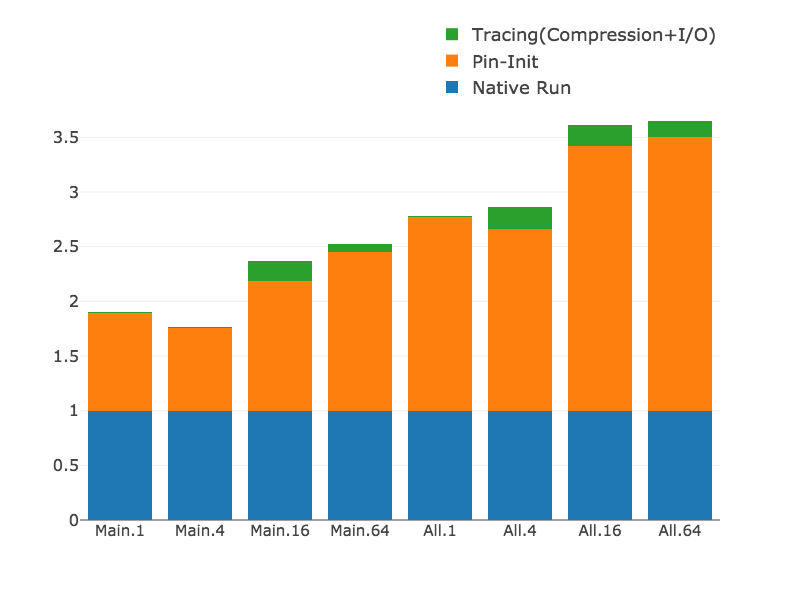
\includegraphics[width=3.1in,height=1.9in]{parlot/figs.comet.newMed/comet_chartDet_B_wc_byTool_p3_5.png}
\caption{ Tracing overhead breakdown - Input B}
\label{comet_chartDet_B_wc_byTool_p3_5}
\end{figure}


\begin{figure}[t]
\centering
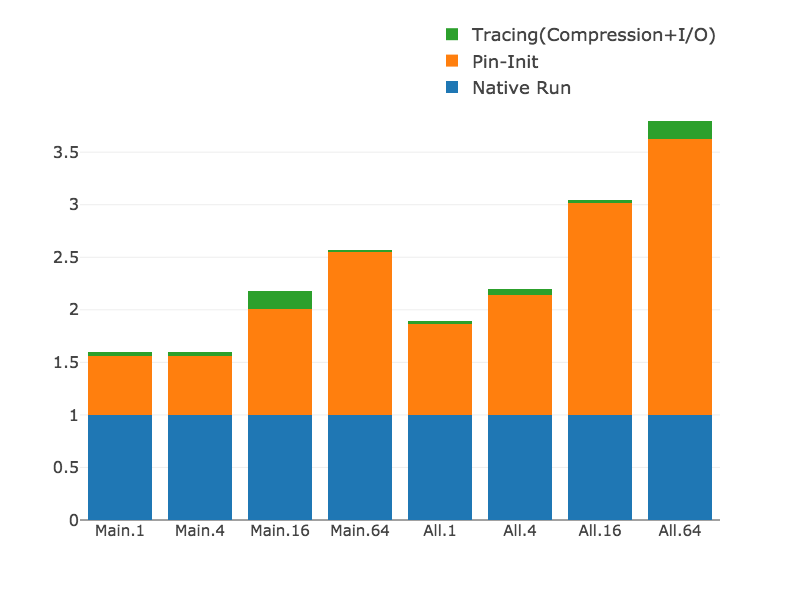
\includegraphics[width=3.1in,height=1.9in]{parlot/figs.comet.newMed/comet_chartDet_C_wc_byTool_p3_5.png}
\caption{ Tracing overhead breakdown - Input C}
\label{comet_chartDet_C_wc_byTool_p3_5}
\end{figure}



\begin{figure}[t]
\centering
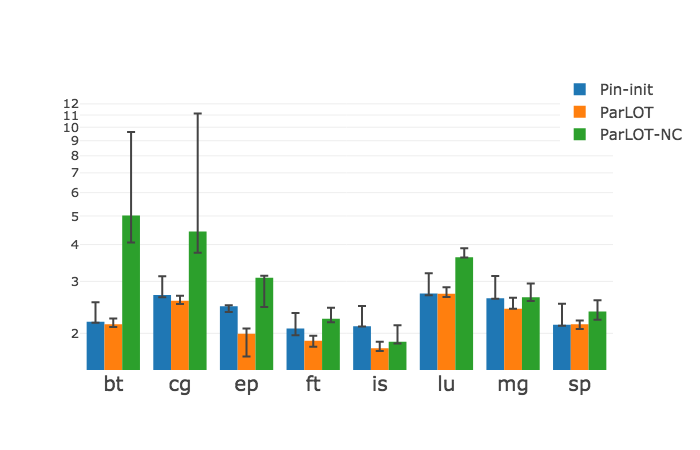
\includegraphics[width=3.2in,height=1.9in]{parlot/figs.comet.newMed/comet_BX2_Main_16_B_p3_5.png}
\caption{ Variability of \parlotm overhead on 16 nodes - Input B}
\label{comet_BX2_Main_16_B_p3_5}
\end{figure}


%%%%%%%%%%%%%%%%%%%%%%%%%%%%%%%%%%%%%%%%%%%%%%%%%%%%%%%%%%%%%%%%%%%%%%%%%%%%%%%%%%

\subsection{Compression Ratio}
\label{subsec:cr}
Table \ref{comet_cr_pMpA_BC_itn_p3.5} shows the compression ratios for all configurations and inputs.
%
On average, \parlot stores between half a kilobyte and a kilobyte of trace information in a single byte.
%
We observe that the
average compression ratio for \parlota on input C is 644.3, and its
corresponding required bandwidth from Table
\ref{comet_bw_pMpAcg_BC_itn_p3.5} is 56.4 kB/s.
%
This means \parlot can
collect \textbf{more than 36 MB} worth of data per core per second
while only needing 56 kB/s of the system bandwidth, {\em leaving the rest of the available bandwidth to the application.}
%
In comparison, \callgrind
collects \textbf{less than 100 kB} of data but still adds more
overhead compared to either \parlota or \parlotm .
%
The average amount of trace data that can be collected by \parlota is
\textbf{360x} (85x for \parlotm) larger than that for \callgrind.
%
In the best observed case, the compression ratio of
\parlot exceeds 21000.
%
This is particularly impressive because it was achieved with relatively low overhead and incremental
on-the-fly compression.
%
Generally, the compression ratios of \parlotm are higher than those of \parlota because the variety of distinct function calls on the main image is smaller than when tracing all images, thus compression performs better on \parlotm.
Also by looking at Fig. \ref{comet_chartAvg_bw_B_p3_5}, Fig. \ref{comet_chartAvg_bw_C_p3_5}, Fig. \ref{comet_chartAvg_cr_B_p3_5} and Fig. \ref{comet_chartAvg_cr_C_p3_5}, we find EP to have the highest compression ratio of the NPB applications. At the same time, it has the minimum required bandwidth. The opposite is true for CG, which exhibits the lowest compression ratio and the highest required bandwidth. CG is a conjugate gradient method with irregular memory accesses and communications whereas EP is an embarrassingly parallel random number generator. CG's whole-program trace contains a larger number of distinct calls and more complex patterns than that of EP, thus resulting in a higher bandwidth and lower compression ratio.
%

\parlot's compression mechanism works better on larger input sizes because larger inputs tend to result in longer streams of similar function calls (e.g., a call that is made for every processed element).



\subsection{Overheads}
\label{subsec:pinit}
Tables \ref{comet_wo_det_Main_all_B_p3.5} and
\ref{comet_wo_det_All_all_B_p3.5} present the average overhead added to each
application for different versions of \parlot.
%
The last row of these two tables
presents the geometric mean.
%
This information captures how much each
phase of \parlot slows down the native execution.

\begin{table}[]
\caption{Tracing overhead of versions of \parlotm - Input B}
\begin{center}
\label{comet_wo_det_Main_all_B_p3.5}
\scalebox{0.5}{
\begin{tabular}{|c|c|rrr|rrr|rrr|rrr|}
\hline
\multicolumn{1}{|l|}{\multirow{2}{*}{\textbf{Input: B}}} & \multicolumn{1}{r|}{Nodes :}    & \multicolumn{3}{c|}{1}  & \multicolumn{3}{c|}{4} & \multicolumn{3}{c|}{16}  & \multicolumn{3}{c|}{64} \\ \cline{2-14}
\multicolumn{1}{|l|}{} & \multicolumn{1}{r|}{Detail Tools:} & \multicolumn{1}{c}{\pininit} & \multicolumn{1}{c}{\parlot} & \multicolumn{1}{c|}{\parlotnc} & \multicolumn{1}{c}{\pininit} & \multicolumn{1}{c}{\parlot} & \multicolumn{1}{c|}{\parlotnc} & \multicolumn{1}{c}{\pininit} & \multicolumn{1}{c}{\parlot} & \multicolumn{1}{c|}{\parlotnc} & \multicolumn{1}{c}{\pininit} & \multicolumn{1}{c}{\parlot} & \multicolumn{1}{c|}{\parlotnc} \\
\hline
\multirow{9}{*}{Main} &     bt  &  1.5  &  1.5  &   5.6  &  1.7  &  1.7  &  5.0  &  2.1  &  2.1  &  5.0  &  1.8  &  2.1  &  3.5 \\
 &  cg  &  1.7  &  1.8  &   2.3  &  1.8  &  1.8  &  2.6  &  2.7  &  2.5  &  4.4  &  2.3  &  2.1  &  4.6 \\
 &  ep  &  2.9  &  2.6  &  20.4  &  1.9  &  1.8  &  5.3  &  2.4  &  1.9  &  3.0  &  2.6  &  2.3  &  2.6 \\
 &  ft  &  1.8  &  2.1  &   6.1  &  1.7  &  1.7  &  2.7  &  2.0  &  1.8  &  2.2  &  2.1  &  1.9  &  2.1 \\
 &  is  &  2.4  &  2.4  &   4.8  &  1.7  &  1.7  &  2.0  &  2.1  &  1.7  &  1.8  &  4.5  &  4.3  &  5.7 \\
 &  lu  &  1.3  &  1.3  &   1.4  &  1.7  &  1.7  &  2.2  &  2.7  &  2.7  &  3.6  &  3.0  &  4.3  &  6.1 \\
 &  mg  &  2.5  &  2.5  &   2.7  &  1.5  &  1.5  &  1.5  &  2.6  &  2.4  &  2.6  &  1.9  &  1.9  &  1.8 \\
 &  sp  &  1.3  &  1.3  &   2.4  &  1.7  &  1.7  &  3.5  &  2.1  &  2.1  &  2.3  &  1.9  &  2.0  &  2.5 \\
\cline{2-14}
 &  GM  &  1.8  &  1.9  &   4.1  &  1.7  &  1.7  &  2.9  &  2.3  &  2.1  &  3.0  &  2.4  &  2.5  &  3.3 \\
\hline
\end{tabular} }

\end{center}
\end{table}








\ignore{--
\begin{table*}[]
\caption{Tracing overhead of different \parlot versions - Input B - Main image}
\begin{center}
\label{comet_wo_det_Main_all_B_p3.5}
\scalebox{0.78}{
\begin{tabular}{|c|c|rrr|rrr|rrr|rrr|}
\hline
\multicolumn{1}{|l|}{\multirow{2}{*}{\textbf{Input: B}}} & \multicolumn{1}{r|}{Nodes :}    & \multicolumn{3}{c|}{1}  & \multicolumn{3}{c|}{4} & \multicolumn{3}{c|}{16}  & \multicolumn{3}{c|}{64} \\ \cline{2-14}
\multicolumn{1}{|l|}{} & \multicolumn{1}{r|}{Detail Tools:} & \multicolumn{1}{c}{\pininit} & \multicolumn{1}{c}{\parlot} & \multicolumn{1}{c|}{\parlotnc} & \multicolumn{1}{c}{\pininit} & \multicolumn{1}{c}{\parlot} & \multicolumn{1}{c|}{\parlotnc} & \multicolumn{1}{c}{\pininit} & \multicolumn{1}{c}{\parlot} & \multicolumn{1}{c|}{\parlotnc} & \multicolumn{1}{c}{\pininit} & \multicolumn{1}{c}{\parlot} & \multicolumn{1}{c|}{\parlotnc} \\
\hline
\multirow{9}{*}{Main} &  bt  &  1.50  &  1.55  &   5.62  &  1.74  &  1.76  &  5.06  &  2.19  &  2.15  &  5.02  &  1.83  &  2.10  &  3.52 \\
 &  cg  &  1.75  &  1.82  &   2.38  &  1.84  &  1.85  &  2.64  &  2.70  &  2.58  &  4.43  &  2.32  &  2.17  &  4.64 \\
 &  ep  &  2.96  &  2.62  &  20.48  &  1.99  &  1.89  &  5.38  &  2.47  &  1.99  &  3.09  &  2.68  &  2.39  &  2.66 \\
 &  ft  &  1.87  &  2.11  &   6.17  &  1.75  &  1.74  &  2.79  &  2.08  &  1.89  &  2.24  &  2.18  &  1.96  &  2.14 \\
 &  is  &  2.47  &  2.47  &   4.82  &  1.79  &  1.78  &  2.07  &  2.11  & 1.78  &  1.87  &  4.51  &  4.31  &  5.71 \\
 &  lu  &  1.32  &  1.31  &   1.44  &  1.75  &  1.77  &  2.25  &  2.73  &  2.73  &  3.62  &  3.05  &  4.39  &  6.13 \\
 &  mg  &  2.56  &  2.53  &   2.79  &  1.56  &  1.52  &  1.59  &  2.63  &  2.43  &  2.65  &  1.95  &  1.97  &  1.85 \\
 &  sp  &  1.34  &  1.33  &   2.43  &  1.73  &  1.73  &  3.58  &  2.14  &  2.15  &  2.37  &  1.95  &  2.07  &  2.54 \\
\cline{2-14}
 &  GM  &  1.89  &  1.90  &   4.10  &  1.77  &  1.75  &  2.92  &  2.37  &  2.19  &  3.00  &  2.45  &  2.52  &  3.33 \\
\hline
\end{tabular} }

\end{center}
\end{table*}
}


\begin{table}[]
\caption{Tracing overhead of versions of \parlota - Input B}
\begin{center}
\label{comet_wo_det_All_all_B_p3.5}
\scalebox{0.78}{
\begin{tabular}{|c|c|rrr|rrr|rrr|rrr|}
\hline
\multicolumn{1}{|l|}{\multirow{2}{*}{\textbf{Input: B}}} & \multicolumn{1}{r|}{Nodes :}    & \multicolumn{3}{c|}{1}  & \multicolumn{3}{c|}{4} & \multicolumn{3}{c|}{16}  & \multicolumn{3}{c|}{64} \\ \cline{2-14}
\multicolumn{1}{|l|}{} & \multicolumn{1}{r|}{Detail Tools:} & \multicolumn{1}{c}{\pininit} & \multicolumn{1}{c}{\parlot} & \multicolumn{1}{c|}{\parlotnc} & \multicolumn{1}{c}{\pininit} & \multicolumn{1}{c}{\parlot} & \multicolumn{1}{c|}{\parlotnc} & \multicolumn{1}{c}{\pininit} & \multicolumn{1}{c}{\parlot} & \multicolumn{1}{c|}{\parlotnc} & \multicolumn{1}{c}{\pininit} & \multicolumn{1}{c}{\parlot} & \multicolumn{1}{c|}{\parlotnc} \\
\hline
\multirow{9}{*}{All} &  bt  &  1.7  &  1.8  &   6.1  &  2.3  &  2.5  &  6.1  &  3.2  &  3.5  &   9.0  &  2.8  &  3.1  &   7.5 \\
 &  cg  &  2.6  &  2.7  &   3.8  &  2.8  &  3.0  &  4.4  &  4.0  &  4.2  &  11.3  &  3.3  & 3.2  &  10.3 \\
 &  ep  &  4.3  &  4.1  &  22.2  &  3.1  &  3.4  &  7.1  &  3.1  &  3.3  &   4.5  &  4.1  & 3.8  &   4.1 \\
 &  ft  &  2.8  &  2.7  &   6.8  &  2.6  &  2.7  &  3.8  &  2.8  &  2.9  &   3.6  &  3.1  &  3.0  &   3.5 \\
 &  is  &  4.4  & 4.2  &   7.0  &  2.8  &  2.9  &  3.4  &  2.9  &  2.8  &   3.2  &  5.3  &  5.4  &   8.8 \\
 &  lu  &  1.7  &  1.7  &   2.3  &  2.5  &  2.7  &  4.8  &  3.9  &  4.3  &  10.4  &  4.4  &  4.6  &  23.4 \\
 &  mg  &  4.8  &  4.7  &   5.3  &  2.5  &  2.7  &  3.0  &  4.3  &  4.4  &   5.2  &  2.7  &  3.1  &   3.2 \\
 &  sp  &  1.7  &  1.7  &   3.0  &  2.4  &  2.6  &  5.0  &  3.2  &  3.6  &   5.6  &  2.7  &  3.3  &  11.6 \\
\cline{2-14}
 &  GM  &  2.7  & 2.7  &   5.5  &  2.6  &  2.8  &  4.5  &  3.4  &  3.6  &   6.0  &  3.5  &  3.6  &   7.4 \\
\hline
\end{tabular} }

\end{center}
\end{table}












\ignore{--

\begin{table}[]
\caption{Tracing overhead of different \parlot versions - Input B}
\begin{center}
\label{comet_wo_det_All_all_B_p3.5}
\scalebox{0.78}{
\begin{tabular}{|c|c|rrr|rrr|rrr|rrr|}
\hline
\multicolumn{1}{|l|}{\multirow{2}{*}{\textbf{Input: B}}} & \multicolumn{1}{r|}{Nodes :}    & \multicolumn{3}{c|}{1}  & \multicolumn{3}{c|}{4} & \multicolumn{3}{c|}{16}  & \multicolumn{3}{c|}{64} \\ \cline{2-14}
\multicolumn{1}{|l|}{} & \multicolumn{1}{r|}{Detail Tools:} & \multicolumn{1}{c}{\pininit} & \multicolumn{1}{c}{\parlot} & \multicolumn{1}{c|}{\parlotnc} & \multicolumn{1}{c}{\pininit} & \multicolumn{1}{c}{\parlot} & \multicolumn{1}{c|}{\parlotnc} & \multicolumn{1}{c}{\pininit} & \multicolumn{1}{c}{\parlot} & \multicolumn{1}{c|}{\parlotnc} & \multicolumn{1}{c}{\pininit} & \multicolumn{1}{c}{\parlot} & \multicolumn{1}{c|}{\parlotnc} \\
\hline
\multirow{9}{*}{All} &  bt  &  1.76  &  1.84  &   6.11  &  2.39  &  2.57  &  6.11  &  3.22  &  3.52  &   9.02  &  2.87  &  3.14  &   7.55 \\
 &  cg  &  2.69  &  2.73  &   3.80  &  2.86  &  3.06  &  4.48  &  4.07  &  4.20  &  11.38  &  3.33  & 3.26  &  10.39 \\
 &  ep  &  4.36  &  4.18  &  22.20  &  3.14  &  3.41  &  7.16  &  3.12  &  3.39  &   4.55  &  4.18  & 3.83  &   4.16 \\
 &  ft  &  2.80  &  2.78  &   6.85  &  2.65  &  2.77  &  3.82  &  2.82  &  2.94  &   3.66  &  3.15  &  3.02  &   3.57 \\
 &  is  &  4.40  & 4.22  &   7.04  &  2.85  &  2.96  &  3.42  &  2.91  &  2.83  &   3.24  &  5.38  &  5.44  &   8.81 \\
 &  lu  &  1.70  &  1.73  &   2.39  &  2.54  &  2.76  &  4.88  &  3.96  &  4.30  &  10.47  &  4.45  &  4.65  &  23.41 \\
 &  mg  &  4.83  &  4.75  &   5.37  &  2.51  &  2.79  &  3.07  &  4.32  &  4.46  &   5.22  &  2.73  &  3.17  &   3.26 \\
 &  sp  &  1.70  &  1.72  &   3.01  &  2.46  &  2.66  &  5.06  &  3.27  &  3.65  &   5.67  &  2.77  &  3.31  &  11.65 \\
\cline{2-14}
 &  GM  &  2.78  & 2.77  &   5.59  &  2.66  &  2.86  &  4.58  &  3.42  &  3.62  &   6.02  &  3.51  &  3.65  &   7.41 \\
\hline
\end{tabular} }

\end{center}
\end{table}
}



%%%%%%%%%%%%%%%%%%%%%%%%%%%%%%%%%%%%%%%%%%%%%%%%%%%%%%%%%%%%%

\begin{figure}[t]
\centering
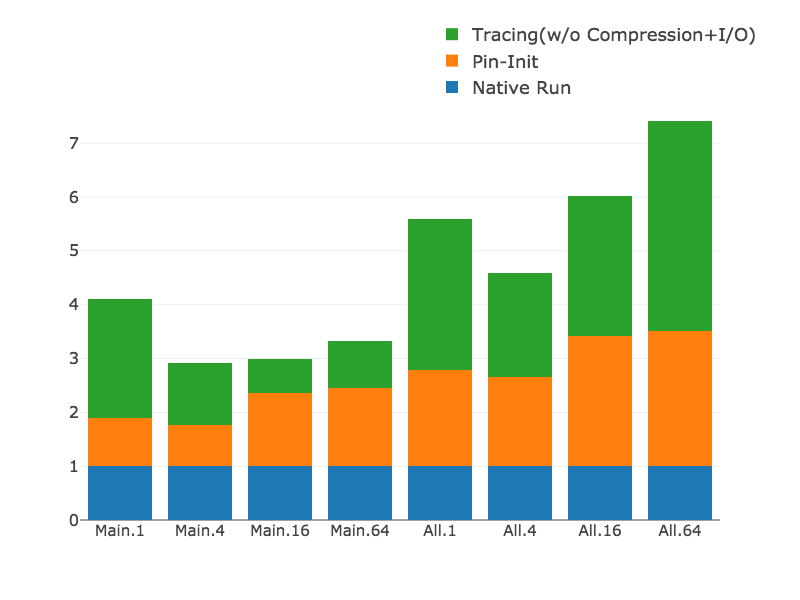
\includegraphics[width=3in,height=1.95in]{parlot/figs.comet.newMed/comet_chartDet_B_woc_byTool_p3_5.png}
\caption{\parlotnc tracing overhead breakdown - Input B}
\label{comet_chartDet_B_woc_byTool_p3_5}
\end{figure}

\begin{figure}[t]
\centering
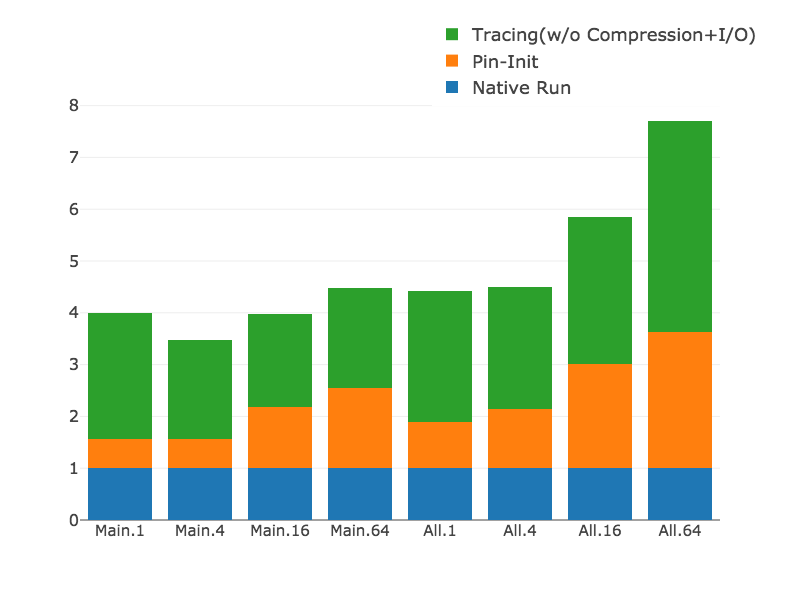
\includegraphics[width=3in,height=1.95in]{parlot/figs.comet.newMed/comet_chartDet_C_woc_byTool_p3_5.png}
\caption{ \parlotnc tracing overhead breakdown - Input C}
\label{comet_chartDet_C_woc_byTool_p3_5}
\end{figure}

In general, one
expects the following inequality to hold:
 the overhead of \pininit should be less than that of \parlot
, which should be less than that of \parlotnc.
%
This is not always the case because of the non-deterministic runtimes of the applications.
%
In fact, the variability across three runs of each experiment
is shown in Fig. \ref{comet_BX2_Main_16_B_p3_5}
where we present the minimum, maximum and median overheads.
%
These
overheads are for input size B and 16 nodes.
%
This variability explains the seeming inconsistencies in  Tables
\ref{comet_wo_det_Main_all_B_p3.5} and
\ref{comet_wo_det_All_all_B_p3.5}.


On average, \pininit adds
an overhead of 3.28  and \parlota adds an overhead of 3.42.
%
This means that \textbf{almost 96\%
of \parlota's overhead is due to \pin}.
%
The results of \parlotm and
other inputs follow the same pattern
as shown in Fig. \ref{comet_chartDet_B_wc_byTool_p3_5} and \ref{comet_chartDet_C_wc_byTool_p3_5}.
%
The overhead that \parlot (excluding the overhead of \pininit) {\em adds}
to the applications is very small.
%
If we were to switch to a different
instrumentation tool that is not as general as \pin but more
lightweight, the overhead would potentially reduce drastically. \\


\subsection{Compression Impact}
\label{subsec:compact}

Fig. \ref{comet_chartDet_B_woc_byTool_p3_5} and Fig. \ref{comet_chartDet_C_woc_byTool_p3_5} show the  overhead breakdown of \parlotnc, which illustrate the impact of compression. They also highlight the importance of incorporating compression directly in the tracing tool.
%
On average, \parlotnc slows down the application execution almost \textbf{2x} more than \parlota.
%
The average overhead
across Table \ref{comet_wo_det_All_all_B_p3.5} for \parlota is \textbf{3.4}.
%
The  corresponding factor for \parlotnc is \textbf{6.6}.
%
The numbers of \parlotm and input C  follow the same pattern. For example, \parlotnc slows down the application execution almost \textbf{1.66x} more than \parlotm.
%

Clearly, compression not only lowers the storage requirement but also the overhead. This is important as it shows that the extra computation to perform the compression is more than amortized by the reduction in the amount of data that need to be written out.
%

This result validates our approach and highlights that incremental, on-the-fly compression is likely essential to make whole-program tracing possible at low overhead.


\section{Discussion and Conclusion}
\label{sec:ch2_concl}

In this paper, 
we present \parlot, a portable low overhead dynamic
binary instrumentation-based
whole-program
tracing approach that can support a variety of 
dynamic program analyses, including debugging.
%
Key properties of \parlot include its on-the-fly trace collection and
compression that reduces timing jitter, I/O bandwidth, and storage requirements to such a degree that whole-program call/return traces can be collected efficiently even at scale. 

We evaluate various versions of \parlot
created by disabling/enabling compression, not collecting any traces, etc.
%
In order to provide an intuitive comparison against a well known tool,
we also compare \parlot to \callgrind.
%
Our metrics include the tracing overhead, required bandwidth, achieved compression ratio, initialization overhead, and the 
overall impact of compression.
%
Detailed evaluations on the NAS parallel benchmarks running on
up to 1024 cores establish the merit of our tool and our design decisions. 
\parlot can collect more than 36 MB worth of data per core per second while 
only needing 56 kB/s of bandwidth and slowing down the 
application by 2.7x on average.
%
These results are highly promising in terms of supporting 
whole program tracing and debugging, in particular when considering that most of the overhead is due to the DBI tool and not \parlot.


The traces collected by \parlot cut through the entire stack of heterogeneous
(MPI, OpenMP, PThreads) calls. 
%
This permits a designer to project these traces onto specific
APIs of interest during program analysis, visualization, and debugging.
%


A number of improvements to \parlot remain to be made.
%
These include allowing users to selectively trace at specific
interfaces: doing so can further increase compression efficiency
by reducing the variety of function calls to be handled by
the compressor.
%
We also discuss the need to bring down initialization overheads, i.e.,
by switching to a less general-purpose DBI tool.
%



\section*{Acknowledgment}

This research was supported by the NSF. We thank our colleague Dr. Hari Sundar from the University of Utah who provided insight and expertise that greatly assisted the research. We also thank the Texas Advanced Computing Center (TACC) and the San Diego Supercomputer Center (SDSC) for the infrastructure they provided for running our experiments.

 
%--end

